\documentclass{standalone}
\usepackage{tikz}
\begin{document}
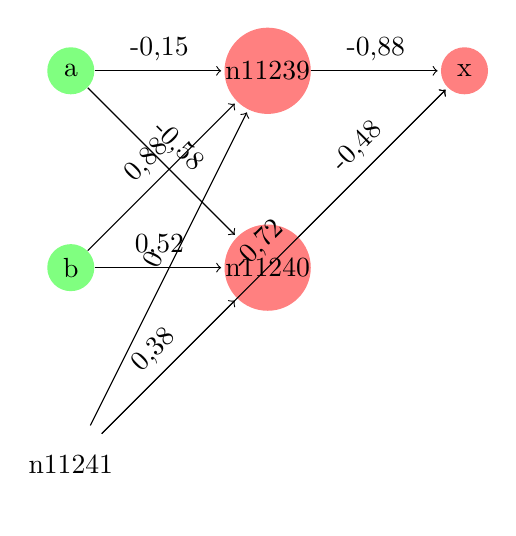
\begin{tikzpicture}[shorten >=1pt,->,draw=black!,node distance=2.5cm]
\tikzstyle{neuron}=[circle,fill=black!25,minimum size=17pt,inner sep=0pt]
\tikzstyle{constant}=[neuron, fill=white!50];
\tikzstyle{identity}=[neuron, fill=green!50];
\tikzstyle{sigmoid}=[neuron, fill=red!50];
\node [identity] (a) {a};
\node [identity,below of=a] (b) {b};
\node [constant,below of=b] (n11241) {n11241};
\node [sigmoid,right of=a] (n11239) {n11239};
\node [sigmoid,below of=n11239] (n11240) {n11240};
\node [sigmoid,right of=n11239] (x) {x};
\path[every node/.style={sloped,anchor=south,auto=false}]
(a) edge node {-0,58} (n11240)
(a) edge node {-0,15} (n11239)
(n11241) edge node {-0,72} (x)
(n11241) edge node {0} (n11239)
(n11241) edge node {0,38} (n11240)
(n11239) edge node {-0,88} (x)
(b) edge node {0,88} (n11239)
(b) edge node {0,52} (n11240)
(n11240) edge node {-0,48} (x)
;\end{tikzpicture}
\end{document}